\documentclass[a4paper,12pt]{article}
\usepackage{school}
\tikzset{
    grid figure/.style={fill=blue!30, draw=black, ultra thick, fill opacity=.5},
    base/.style={circle, draw=black, inner sep=0pt, minimum size=3mm, fill opacity=1},
    inner/.style={fill=white, base},
    outer/.style={fill=black, base},
}

\begin{document}
    \head{19 марта}{Площади на клетчатой бумаге}
    \iirules
    
    Все площади в этом листке измеряются в клеточках. Вершины всех многоугольников, если не сказано обратного, находятся в узлах сетки. \\
    \defn Прямоугольник называется \emph{клетчатым}, если его стороны проходят по линиям сетки. \\
    
    \problem Найдите площади фигур на рисунке. \\
    \begin{center}
        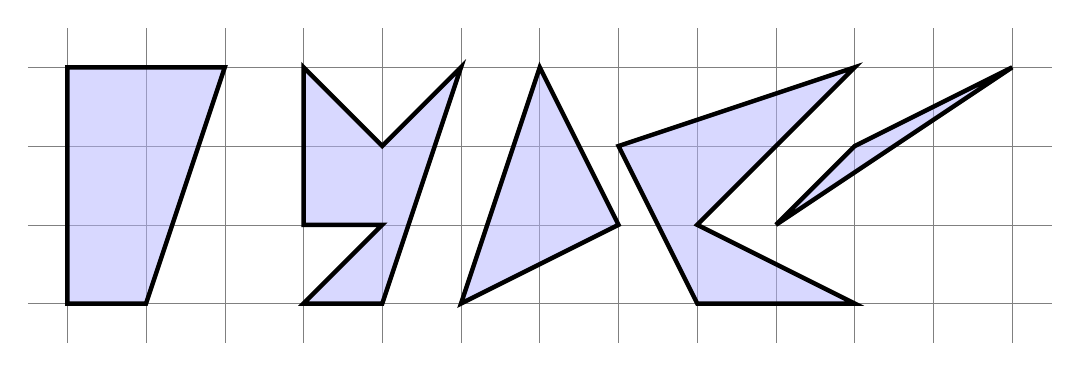
\begin{tikzpicture}
            \draw[help lines] (-.5,-.5) grid (12.5,3.5);
            \draw[grid figure] (0,0) -- (1,0) -- (2,3) -- (0,3) -- cycle;
            \draw[grid figure] (3,0) -- (4,0) -- (5,3) -- (4,2) -- (3,3) -- (3,1) -- (4,1) -- cycle;
            \draw[grid figure] (5,0) -- (7,1) -- (6,3) -- cycle;
            \draw[grid figure] (8,0) -- (10,0) -- (8,1) -- (10,3) -- (7,2) -- cycle;
            \draw[grid figure] (9,1) -- (12,3) -- (10,2) -- cycle;
            \node[below left] at (0,3) {\sub};
            \node[below left] at (3,3) {\sub};
            \node[below left] at (6,3) {\sub};
            \node[below left] at (8,3) {\sub};
            \node[below left] at (11,3) {\sub};
        \end{tikzpicture}
    \end{center}
    
    \problem На клетчатой бумаге отмечены вершины квадрат $4 \times 4$. Отметьте еще два узла сетки и соедините их замкнутой ломаной так, чтобы получился шестиугольник площади 6 клеток.
    \problemw Докажите, что площадь \sub треугольника; \sub четырехугольника с вершинами в узлах сетки либо целая, либо полуцелая.
    \begin{solution}
        \sub Впишем данный треугольник (далее --- $T$) в клетчатый прямоугольник. Для этого достаточно провести вертикальные прямые через самую правую и самую левую вершины треугольника и горизонтальные прямые через самую нижнюю и самую верхнюю вершины треугольника. Если все вершины $T$ оказались на сторонах прямоугольника, то площадь прямоугольника равна сумме площадей $T$ и трёх прямоугольных треугольников $ADC$, $CEB$ и $BFA$. Если же какая-то вершина $C$ треугольника $T$ не лежит на стороне прямоугольника, проведём из неё вертикальный и горизонтальный отрезки до сторон прямоугольника, не пересекающие $T$. Тогда площадь прямоугольника равна сумме площадей $T$, клетчатого прямоугольника $BGFH$ и трёх прямоугольных треугольников $ADC$, $CGB$ и $BHA$. Следовательно, площадь $T$ полуцелая. \\
        \sub Разделим четырёхугольник диагональю на два треугольника. Так как площадь каждого из треугольников полуцелая, площадь четырёхугольника также полуцелая.
        \begin{center}
            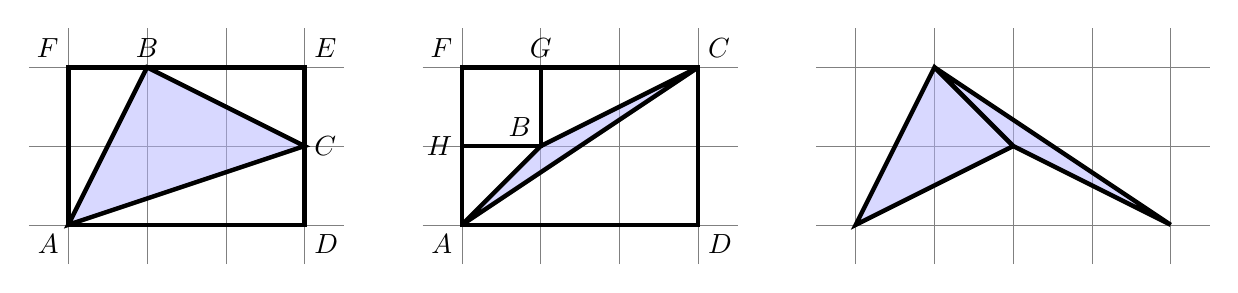
\begin{tikzpicture}
                \begin{scope}
                    \draw[help lines] (-.5,-.5) grid (3.5,2.5);
                    \draw[grid figure] (0,0) -- (3,1) -- (1,2) -- cycle;
                    \draw[ultra thick] (0,0) -- (3,0) -- (3,2) -- (0,2) -- cycle;
                    \node[below left] at (0,0) {$A$};
                    \node[above] at (1,2) {$B$};
                    \node[right] at (3,1) {$C$};
                    \node[below right] at (3,0) {$D$};
                    \node[above right] at (3,2) {$E$};
                    \node[above left] at (0,2) {$F$};
                \end{scope}
                \begin{scope}[xshift=5cm]
                    \draw[help lines] (-.5,-.5) grid (3.5,2.5);
                    \draw[grid figure] (0,0) -- (3,2) -- (1,1) -- cycle;
                    \draw[ultra thick] (0,0) -- (3,0) -- (3,2) -- (0,2) -- cycle (0,1) -- (1,1) -- (1,2);
                    \node[below left] at (0,0) {$A$};
                    \node[above left] at (1,1) {$B$};
                    \node[above right] at (3,2) {$C$};
                    \node[below right] at (3,0) {$D$};
                    \node[above left] at (0,2) {$F$};
                    \node[above] at (1,2) {$G$};
                    \node[left] at (0,1) {$H$};
                \end{scope}
                \begin{scope}[xshift=10cm]
                    \draw[help lines] (-.5,-.5) grid (4.5,2.5);
                    \draw[grid figure] (0,0) -- (2,1) -- (1,2) -- cycle;
                    \draw[grid figure] (4,0) -- (2,1) -- (1,2) -- cycle;
                \end{scope}
            \end{tikzpicture}
        \end{center}
    \end{solution}
    
    \illustrated{
        \draw[help lines] (-.5,-.5) grid (3.5,2.5);
        \draw[grid figure] (0,0) node[outer]{} -- (1,0) node[outer]{} -- (2,0) node[outer]{} -- (3,0) node[outer]{} -- (3,1) node[outer]{} -- (3,2) node[outer]{} -- (2,2) node[outer]{} -- (1,2) node[outer]{} -- (0,2) node[outer]{} -- (0,1) node[outer]{} -- cycle;
        \node[inner] at (1,1) {};
        \node[inner] at (2,1) {};
        \node[below] at (1.5,-.5) {$i = 2, b = 10$};
    }{
        \problemw \sub Выразите площадь клетчатого прямоугольника со стороной 1 через количество узлов сетки на его границе. \\
        \sub Выразите площадь клетчатого прямоугольника через количество $i$ узлов сетки внутри него и количество $b$ узлов сетки на его границе.
    }
    \begin{solution}
        \sub Пусть стороны клетчатого прямоугольника равны $1$ и $y$. Тогда количество узлов сетки $b$ на его границе равно $2 \cdot (y + 1)$. Следовательно, площадь прямоугольника равна $1 \cdot y = \dfrac{b}{2} - 1$. \\
        \sub Пусть стороны клетчатого прямоугольника равны $x$ и $y$. Тогда количество узлов сетки $b$ на его границе равно $2 \cdot (x + 1) + 2 \cdot (y + 1) - 4 = 2x + 2y$, а количество узлов сетки $i$ внутри него равно $(x + 1) \cdot (y + 1) - b = xy - x - y + 1$. Следовательно, площадь прямоугольника равна $x \cdot y = i + \dfrac{b}{2} - 1$.
    \end{solution}

    \illustrated{
        \draw[help lines] (-.5,-.5) grid (3.5,3.5);
        \draw[grid figure] (1,0) node[outer]{} -- (2,0) node[outer]{} -- (3,0) node[outer]{} -- (2,1) node[outer]{} -- (3,3) node[outer]{} -- (2,3) node[outer]{} -- (1,2) node[outer]{} -- (0,3) node[outer]{} -- cycle;
        \node[inner] at (1,1) {};
        \node[inner] at (2,2) {};
        \node[below] at (1.5,-.5) {$i = 2, b = 8$};
    }{
        \begin{theorem}[Формула Пика]
            Площадь многоугольника с вершинами в узлах сетки равна $i + \dfrac{b}{2} - 1$, где $i$ --- количество узлов сетки внутри него и $b$ --- количество узлов сетки на его границе.
        \end{theorem}
    }
    
    \problemw Докажите формулу Пика \sub для прямоугольного треугольника с катетами, идущими по линиям сетки; \sub для любого треугольника, одна из сторон которого идет по линиям сетки.
    \problem \sub Если многоугольник с вершинами в узлах сетки разрезан на две части, для каждой из которых верна формула Пика, то формула Пика верна и для всего многоугольника. \\
    \sub Формула Пика верна для любого треугольника. \\
    \sub Формула Пика верна для любого многоугольника.
    \begin{solution}
        \illustrated{ % TODO починить подписи
        \newcommand{\ravno}{=}
            \draw[help lines] (-.5,-.5) grid (4.5,2.5);
            \draw[grid figure] (0,0) node[outer]{} -- (1,0) node[outer]{} -- (2,0) node[outer]{} -- (3,0) node[outer]{} -- (4,0) node[outer, label=above:$A$]{} -- (2,1) node[outer, label=above:$h\ravno3$]{} -- (0,2) node[outer, label=above:$B$]{} -- (0,1) node[outer]{} -- cycle;
        }{
            \sub Пусть $h$ --- число узлов сетки на гипотенузе, $s$ --- площадь треугольника. Достроим треугольник до прямоугольника $R$ площади $2s$. Тогда число узлов сетки $i_R$ внутри $R$ равно $2i + h - 2$ (2 "лишних" --- $A$ и $B$), а число узлов сетки $b_R$ на границе $R$ равно $2(b - h) + 2$ (2 "дополнительных" --- опять же $A$ и $B$). Следовательно, по доказанной формуле Пика для прямоугольника имеем
            \begin{equation*}
                2s = i_R + \frac{b_R}{2} - 1 = 2i + h - 2 + \frac{2(b - h) + 2}{2} - 1 = 2i + b - 2.
            \end{equation*}
            Отсюда $s = \dfrac{2i + b - 2}{2} = i + \dfrac{b}{2} - 1$, что и требовалось.
        } \\
        \sub TODO
    \end{solution}

    \illustrated{
        \draw[help lines] (-.5,-.5) grid (6.5,3.5);
        \draw[thick] (1/3,-.5) -- (1,0) -- (5,3) -- (5+2/3,3.5);
        \node[outer] at (3,2) {};
    }{
        \problemw Найдите расстояние от точки до прямой.
    }
\end{document}